\documentclass[11pt,a4paper]{jsarticle}
%
\usepackage{listings,jlisting}
\usepackage{amsmath,amssymb}
\usepackage{bm}
\usepackage{ascmac}
\usepackage[dvipdfmx]{graphicx}
\usepackage{here}
%ここからソースコードの表示に関する設定
\lstset{
  basicstyle={\ttfamily},
  identifierstyle={\small},
  commentstyle={\smallitshape},
  keywordstyle={\small\bfseries},
  ndkeywordstyle={\small},
  stringstyle={\small\ttfamily},
  frame={tb},
  breaklines=true,
  columns=[l]{fullflexible},
  numbers=left,
  xrightmargin=0zw,
  xleftmargin=3zw,
  numberstyle={\scriptsize},
  stepnumber=1,
  numbersep=1zw,
  lineskip=-0.5ex
}
%ここまでソースコードの表示に関する設定
\begin{document}


\title{計数工学プログラミング演習最終レポート}
\author{計数工学科システム情報学コース3年\\03-190615\\工藤龍}
\maketitle

\section{課題内容}

疎行列の2乗を様々な手法で計算し,実行時間を測定した.

\section{手法}

今回の実験に用いたのは,以下の4つのアルゴリズムである.
\begin{itemize}
\item dense_ijk
\item dense_ikj
\item sparce_transpose
\item sparce_access
\end{itemize}
以下,上記の四つの説明をする.
dense_ijkは,二次元配列の形で行列を保持するアルゴリズムである.
次のような形で積を計算する.
\begin{lstlisting}
for (int i = 0; i < n; i++) {
    for (int j = 0; j < m; j++) {
        x = 0;
        for (int k = 0; k < n; k++) {
            x += A[i][k] * A[k][j];
        }
        M[i][j] = x;
    }
}
\end{lstlisting}

dense_ikjは,同じように二次元配列の形で行列を保持するが,積の計算の順序がやや異なる.
具体的には以下のようになっている.
\begin{lstlisting}
for (int i = 0; i < n; i++) {
    for (int k = 0; k < n; k++) {
        for (int j = 0; j < m; j++) {
            M[i][j] += A[i][k] * A[k][j];
        }
    }
}
\end{lstlisting}

sparce_transposeは,隣接リストの形で行列を保持するものである.
入力した行列と,その転置行列を考えることで計算する方針をとっている.

sparce_accessは,transposeと同様に隣接リストで行列を保持するが,
access関数を用いることで,転置を考えずに直接積を計算している.

\section{実験結果}

\begin{figure}[H]
  \begin{center}
  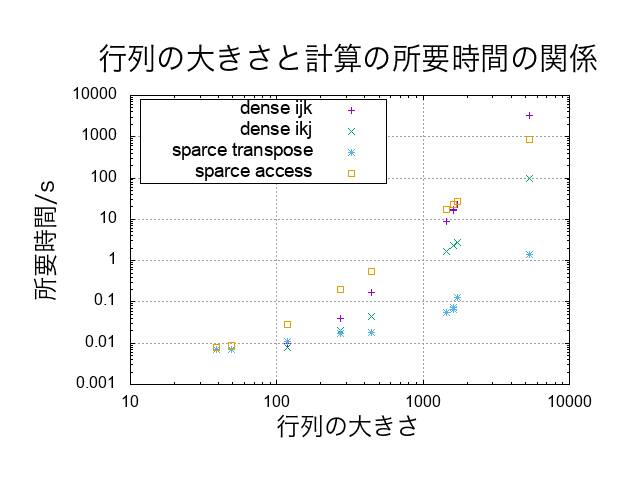
\includegraphics[width=10cm]{../graph.png}
  \end{center}
\end{figure}


\section{考察}

解説文を読んで,このソースをいろいろと変更してみましょう。

\end{document}
